\documentclass[spanish]{beamer}

%%% CODIFICACIÓN

\usepackage[utf8]{inputenc}
\usepackage[spanish]{babel}
\usepackage{graphics,tikz}
\graphicspath{{./fig/}}
%%% FUENTES

\usepackage[T1]{fontenc}
\usepackage[familydefault,regular]{}
\usepackage{newtxsf} % Fuente de matemáticas

\setbeamertemplate{navigation symbols}{}

%%% COLORES

\definecolor{background}{RGB}{255,255,255}
\definecolor{text}{RGB}{78,78,78}
\definecolor{accent}{RGB}{6, 105, 125}

\setbeamerfont{framesubtitle}{size=\normalfont\tiny}
\setbeamercolor{framesubtitle}{fg=white}

%%% Matemáticas
\usepackage{amsmath}
\usepackage{amssymb}
\usepackage{amsbsy}
\usepackage{tipa}
\newcommand{\norm}[1]{\left\lVert#1\right\rVert}
\newcommand{\yy}{\textbf{y}}

%%% AJUSTES DE BEAMER

% ¿Negrita en el título de diapositiva o no?
%\setbeamertemplate{frametitle}{\color{accent}\vspace*{1cm}\bfseries\insertframetitle\par\vskip-6pt}

\setbeamertemplate{frametitle}{\color{accent}\vspace*{1cm}\insertframetitle\par\vskip-6pt}

\setbeamertemplate{itemize items}[circle] % Viñetas de itemize

%%% CONFIGURACIÓN DE COLORES DE BEAMER

\setbeamercolor{background canvas}{bg=background}
\setbeamercolor{normal text}{fg=text}
\setbeamercolor{alerted text}{fg=accent}
\setbeamercolor{block title}{fg=accent}
\setbeamercolor{alerted text}{fg=accent}
\setbeamercolor{itemize item}{fg=accent}
\setbeamercolor{enumerate item}{fg=accent}
\setbeamercolor*{title}{fg=accent}
\setbeamercolor{caption name}{fg=accent}
\setbeamercolor{qed symbol}{fg=accent}
\setbeamercolor{itemize subitem}{fg=accent}
\setbeamercolor{bibliography entry author}{fg=text}
\setbeamertemplate{itemize subitem}[triangle]
\usebeamercolor[fg]{normal text}

%%% INFORMACIÓN DEL DOCUMENTO

\title{\textit{Clustering}}
\subtitle{Estadística Multivariante}
\author{Sofía Almeida Bruno\\ Daniel Bolaños Martínez\\ José María Borrás Serrano\\ Fernando de la Hoz Moreno\\ Pedro Manuel Flores Crespo\\ María Victoria Granados Pozo}


\begin{document}

\maketitle
	
\begin{frame}{\textit{Clustering}}
  \begin{itemize}
  \item Objetivo: agrupar objetos similares.
  \item Dadas \textbf{$x_1$}$,\cdots, $\textbf{$x_n$} medidas de $p$ variables en $n$ objetos considerados \textit{heterogéneos}. El objetivo del análisis clúster es agrupar estos objetos en $k$ clases \textit{homogéneas}, donde $k$ es también desconocido.
  \end{itemize}
\end{frame}

\begin{frame}{\textit{Clustering}}
\begin{figure}[H]
	\centering
	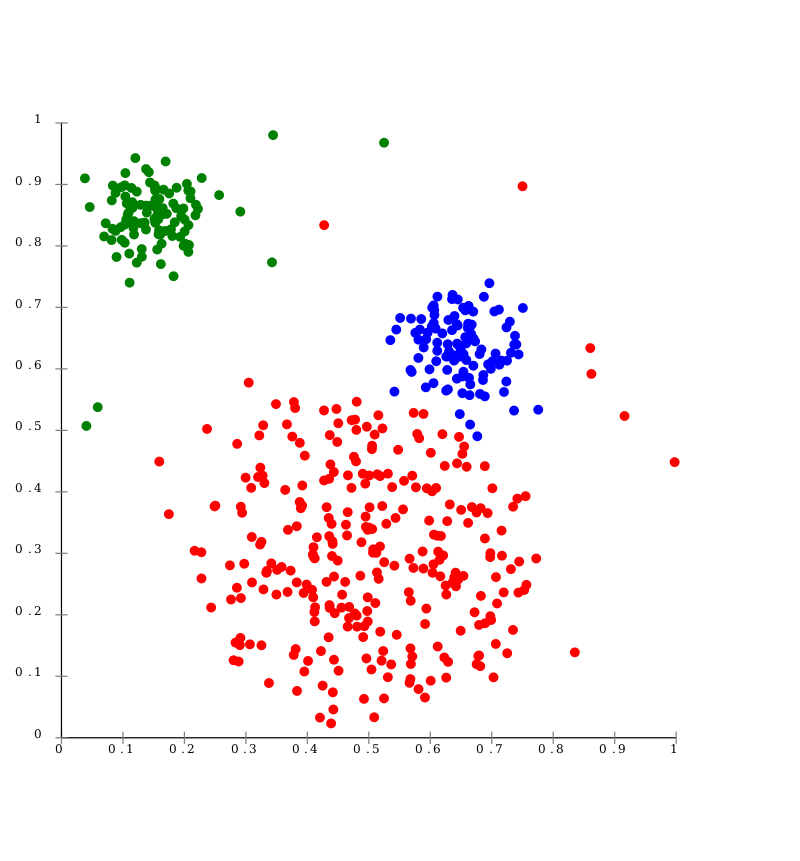
\includegraphics[scale=0.2]{ejemplo}
	\caption{Ejemplo de \textit{clustering}. \cite{chire_deutsch:_2011}}
	\label{fig:ejemplo1}
\end{figure}
\end{frame}

\begin{frame}{Ejemplos de \textit{Clustering}}
  \begin{itemize}
  \item Biología: determinación de especies.
  \item \textit{Marketing}: descubrimiento de grupos de clientes.
    \begin{figure}[H]
	\centering
	
\includegraphics[scale=0.5]{ej_marketing}
	\caption{Ejemplo de \textit{clustering}. \cite{noauthor_understanding_nodate}}
\end{figure}
  \item Psicología: encontrar tipos de personalidad.
  \item Arqueología: datar objetos encontrados.
  \item Planificación urbana: identificar grupos de viviendas.
  \end{itemize}
\end{frame}

\begin{frame}{\textit{Clustering}}
  Para realizar un análisis clúster hay que:
  \begin{itemize}
  \item Elegir una medida de similitud.
  \item Elegir un algoritmo para construir los grupos.
    \begin{itemize}
    \item Particionamiento.
    \item Jerárquicos.
    \end{itemize}
  \end{itemize}
\end{frame}

\section{Número de clústeres}

\begin{frame}{Número de clústeres}
	\begin{itemize}
		\item En los algoritmos de \textit{clustering}, uno de los problemas es determinar el número idóneo de clústeres $ k $. 
		\item Es un proceso ambiguo. Depende de las interpretaciones según la forma y la escala de de la distribución de los datos y la solución deseada.
		\item Como $ k $ decrece de $ n $ a 1, el valor de la distancia debería aumentar ya que tendría que ser mayor cuando dos clústeres distintos se agrupan en uno solo.
	\end{itemize}
\end{frame}

\begin{frame}{Número de clústeres-Método del codo}
	Consiste en dibujar la gráfica de las distancia a los centros de cada clúster en función del número de clústeres. Definimos:
	\[
	SSE_k = \sum_{i = 1}^{n_k} = \norm{\yy_i - \bar{\yy}_k}^2,
	\]
	y para cada $ k $ dibujamos
	\[
	D_k = \sum_{i = 1} ^ {k} SSE_k.
	\]
\end{frame}

\begin{frame}{Número de clústeres-Método del codo}
	\begin{figure}[h]
		\centering
		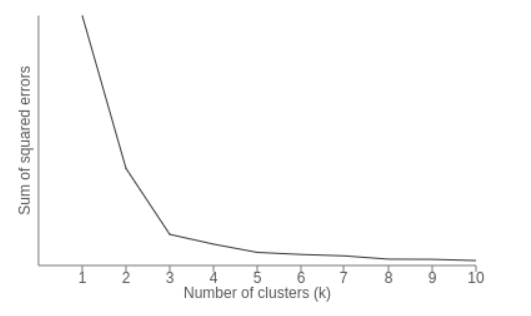
\includegraphics[scale=0.5]{pedro/elbowGraph}
		\caption{Ejemplo del método del codo.}
		\label{smkm}
	\end{figure}
\end{frame}

\begin{frame}{Número de clústeres-Estadístico $ R^2 $}
	Para $ n $ clústeres la suma total de las distancias al cuadrado es $ T = \sum_{i = 1}^{n} \norm{\yy_i - \bar{\yy}}^2 $. Así, para $ k $ clústeres definimos $ R^2 $ como
	\[
	R^{2}_{k} = \frac{T - \sum_k SSE_k}{T}.
	\]
	Para $ n $ clústeres $ SSE_k = 0 $ por lo que $ R^2 = 1 $. Una gran disminución en $ R^2_k $ representaría un agrupamiento diferente. \\
	También podríamos tener en cuenta el cambio en $ R^2 $ al unir los clústeres $ R $ y $ S $ como $ SR^2 = R_k^2 - R^2_{k-1} $. El estadístico $ SR^2 $ representa, en función de $ T $, la proporción de $ SSE_t - (SSE_r + SSE_s) $ donde los clústeres $ C_R $ y $ C_S $ se han unido para formar el clúster $ C_T $.  Cuanto mayor sea el índice mayor será la pérdida de homogeneidad.
\end{frame}

\begin{frame}{Número de clústeres-Varianza agrupada}
	Para un solo clúster \[ s^2 = \sum_{i=1}^{n} \norm{\yy_i - \bar{\yy}}^2/ p(n-1).\]
	Para el clúster $ C_k $
	\[
	s^2 = \sum_{i=1}^{n_k} \norm{\yy_i - \bar{\yy}_k}^2/ p(n_k-1).
	\]
	Valores grandes de la varianza agrupada indica que los clústeres no son homogéneos. Por lo tanto, si tiende a cero para algún $  k < n $ indica la formación de un clúster homogéneo.
\end{frame}

\begin{frame}{Número de clústeres-Pseudo estadísticos}
	El pseudo estadístico $ F $ se define como
	\[
	F^*_k = \frac{(T-\sum_k SSE_k) / (k-1)}{\sum_k SSE_k / (n-k)}.
	\]
	El pseudo estadístico $ t^2 $ se define como
	\[
	\text{pseudo }t^2 = \frac{\lbrack SSE_t - (SSE_r + SSE_s)\rbrack(n_R + n_S - 2)}{SSE_r + SSE_s}.
	\]
\end{frame}

\begin{frame}{Número de clústeres-\textit{Silhouette method}}
	Definimos el índice:
	\[
	s(i) = \frac{b(i)-a(i)}{\max\{b(i), a(i)\}}, \hspace{2mm} \forall i = 1, \dots, n
	\] 
	donde 
	\[
	a(i) = \frac{1}{|C_i|-1}\sum_{j\in C_i, j \neq i} d(i,j) 
	\]	y
	\[
	b(i) = \min_{k \neq i} \frac{1}{|C_k|} \sum_{j \in C_k} d(i,j).
	\] 
	Se escoge el $ k $ que maximice el valor medio de $ s(i) $.
\end{frame}

\begin{frame}{Número de clústeres-\textit{Silhouette method}}
	\begin{table}[h!]
		\centering
		\begin{tabular}{cc} 
			\hline
			k & Silhouette coeff. \\
			\hline
			2 &  0.7049787496083262 \\			 
			3 & 0.5882004012129721 \\	
			4 &  0.6505186632729437 \\
			5 &  0.5745566973301872 \\
			6 & 0.43902711183132426 \\
			\hline
		\end{tabular}
		\caption{Ejemplo \textit{silhouette method}.}
	\end{table}
	Vemos que se obtienen los mejores resultados con 2 o 4 clústeres.
\end{frame}

\begin{frame}{Número de clústeres-\textit{Gap method}}
	El $ k $ elegido será aquel que maximice el valor de:
	\[
	Gap(k) = E^*_n\{ \log(W_k)\} - \log(W_k).
	\]
	En la fórmula anterior $ E^*_n $ denota la media de una de muestra de tamaño $ n $ y 
	\[
	W_k = \sum_{R = 1}^{k}\frac{1}{2 n_R}\sum_{i j \in C_R} d(i,j).
	\]
\end{frame}

\begin{frame}{Número de clústeres-\textit{Gap method}}
	\begin{figure}[H]
		\centering
		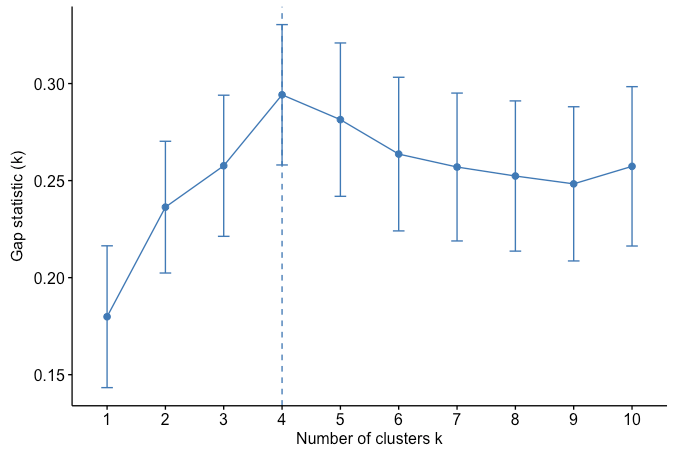
\includegraphics[scale=0.32]{pedro/gapGraph}
		\caption{Ejemplo del método de la brecha.}
	\end{figure}
\end{frame}

\begin{frame}[fragile, allowframebreaks]
  \frametitle{Referencias}
%  \nocite{*}
        \bibliographystyle{amsalpha}
        \bibliography{referencias_pres.bib}
\end{frame}
\end{document}

